\documentclass{config}
\usepackage[T1]{fontenc}
\usepackage[utf8]{inputenc}
\usepackage{graphicx}
\usepackage{color}
\usepackage{siunitx}
\usepackage{listings}
\usepackage{wrapfig}
\usepackage{subcaption}
\usepackage{float}
\usepackage[toc,page]{appendix} 
\usepackage{amsmath}
\usepackage{bigints}
\usepackage{multicol}
\newcommand\x{\XSolid}

\usepackage[labelfont=sc]{caption}
\title{Intracranial pressure}
%\author{Jeanne VENTRE}

%\instlabel{}{Master 2 of Engineering in Fluid Mechanics Fundamentals and Applications, Pierre and Marie Curie University (UPMC)}

\begin{document}

\maketitle

\begin{figure}[H]
\centering
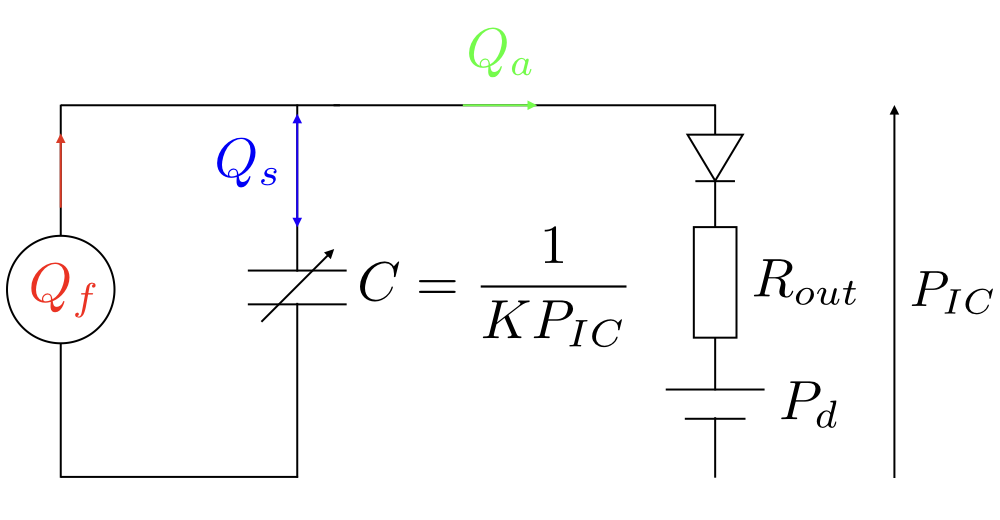
\includegraphics[scale=0.3]{modele0D.png}
\caption{Drawing of the cerebrospinal fluid system described as an electrical analogy.}
\label{schema0D}
\end{figure}

\begin{equation}\label{compliance}
C = \frac{1}{K P_{IC}}
\end{equation}

Conservation of mass requires:

\begin{equation}\label{debit}
Q_f = Q_a + Q_s
\end{equation}

\begin{equation}\label{q_absorption}
Q_a = \frac{P_{IC} - P_d }{R_{out}}
\end{equation}

\begin{equation}\label{Pd}
P_d = P_r - Q_f ~ R_{out}
\end{equation}

where $P_r$ is the resting pressure, $P_d$ is the dural venous pressure.

\begin{equation}\label{edo1}
\frac{\mathrm{d}P_{IC}}{\mathrm{d}t} = K ~ P_{IC} ~ Q_s = K ~ P_{IC } ~ (Q_f - Q_a)
\end{equation}

Substituting Eq. (\ref{q_absorption}) in (\ref{edo1}): 

\begin{equation}\label{edo_final}
\frac{\mathrm{d}P_{IC}}{\mathrm{d}t} = K ~ P_{IC } ~ Q_f - K ~ P_{IC}  \frac{P_{IC} - P_d }{R_{out}}
\end{equation}

Analytic solution for Eq. (\ref{edo_final}) is the following:

\begin{equation}\label{sol_analytic}
P_{IC}(t) = \frac{P_p e^{\frac{K t P_r}{R_{out}}}}{1 + \frac{P_p}{P_r}\left(e^{\frac{K t P_r}{R_{out}}} - 1 \right) }
\end{equation}

Discretizing with an explicit Euler scheme leads to:

\begin{equation}\label{Euler_explicit}
P_{IC} ^{n+1} = P_{IC} ^n  + \Delta t  ~ K ~ P_{IC}^n \left(Q_f^n - \frac{P_{IC}^n - P_d}{R_{out}}\right)
\end{equation}


\begin{table}[H]
\begin{center}
\begin{tabular}{|c|c|c|}
\hline 
$Q_f$ & 0.36 mL/min \\
\hline 
$K$ & 0.5 mL \\
\hline 
$R_{out}$ & 7.5 mmHg / (mL/min) \\ 
\hline 
$P_r$ & 30 mmHg \\ 
\hline 
$P_{IC}(0)$ & 8 mmHg \\ 
\hline
\end{tabular} 
\caption{Parameters of the model}
\label{parameters}
\end{center}
\end{table}

\begin{figure}[H]
\centering
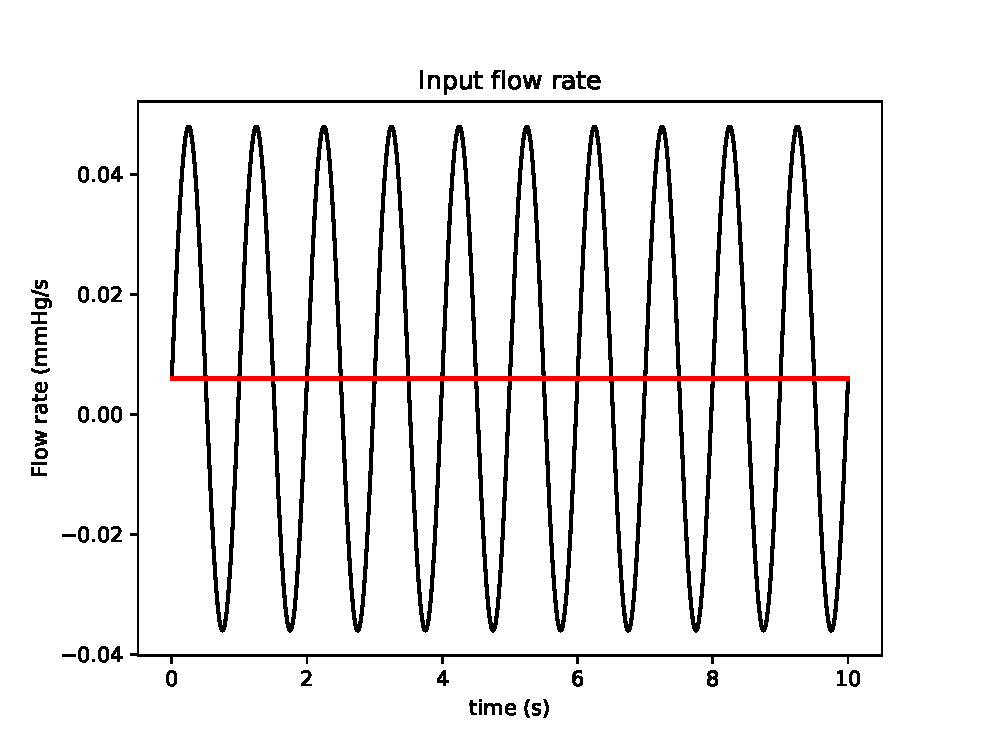
\includegraphics[scale=0.55]{flow.eps}
\caption{Pulse input $Q_f$ (in black) and constant input flow $Q_f$ (in red) as a function of time.}
\label{input_flow}
\end{figure}

\begin{figure}[H]
\begin{minipage}{.48\textwidth}
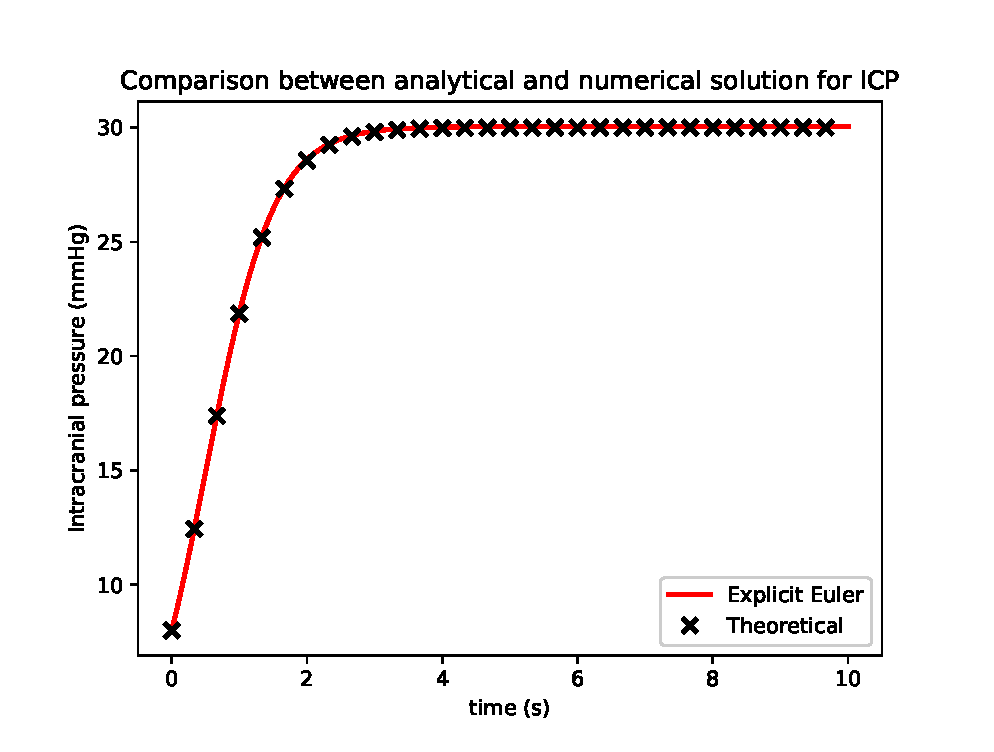
\includegraphics[scale=0.55]{icp_constant.eps}
\end{minipage} \hfill
\begin{minipage}{.48\textwidth}
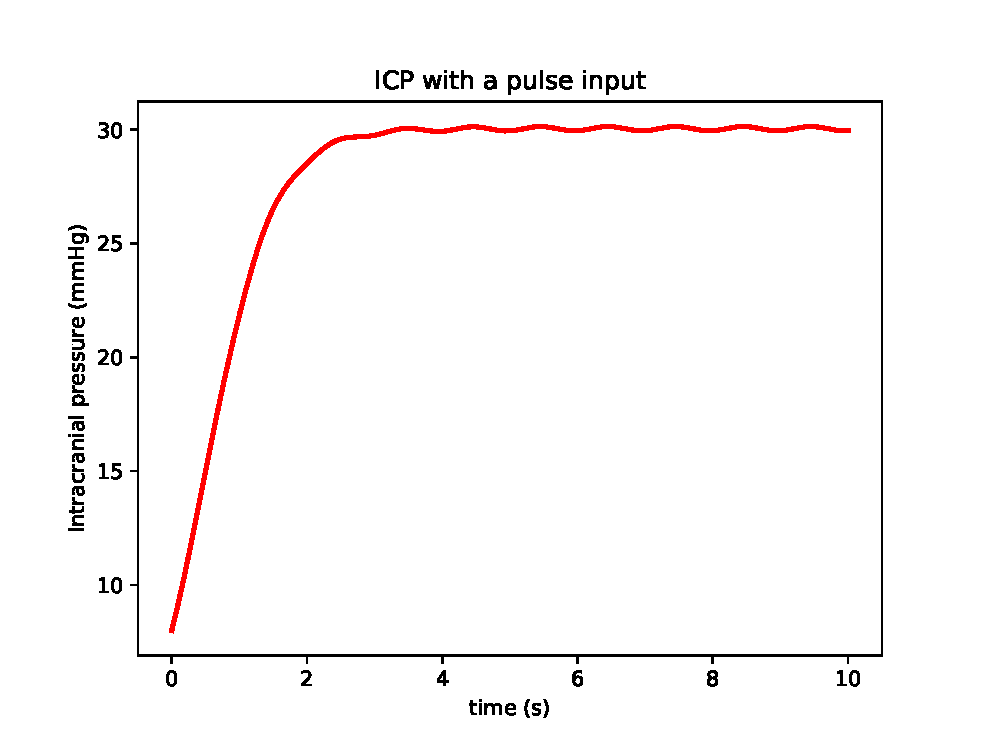
\includegraphics[scale=0.55]{icp_pulse.eps}
\end{minipage}
\caption{Intracranial pressure (in mmHg) as a function of time (in s) for two different $Q_f$. Left: comparison between analytical solution (\ref{sol_analytic}) and numerical solution of Eq. (\ref{Euler_explicit}) with a constant $Q_f$. Right: numerical solution of Eq. (\ref{Euler_explicit}) for intracranial pressure with a pulse $Q_f$. }
\end{figure}

\begin{figure}[H]
\centering
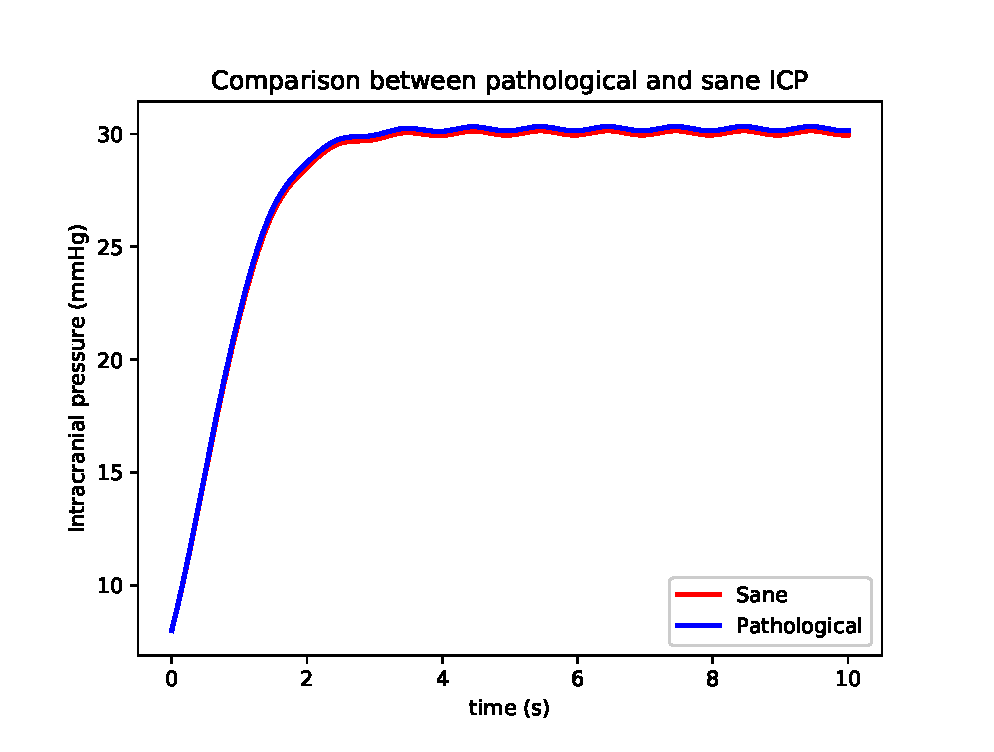
\includegraphics[scale=0.55]{icp_patho.eps}
\caption{Intracranial pressure (in mmHg) for sane (red) and pathological (blue)}
\end{figure}

\nocite{*}
\bibliographystyle{plain}
\bibliography{biblio}


\end{document}
